\documentclass{article}
\usepackage[utf8x]{inputenc}
\usepackage{ucs}
\usepackage{amsmath} 
\usepackage{amsfonts}
\usepackage{upgreek}
\usepackage[english,russian]{babel}
\usepackage{graphicx}
\usepackage{float}
\usepackage{textcomp}
\usepackage{hyperref}
\usepackage{geometry}
  \geometry{left=2cm}
  \geometry{right=1.5cm}
  \geometry{top=1cm}
  \geometry{bottom=2cm}
\usepackage{tikz}
\usepackage{ccaption}
\usepackage{multicol}

\usepackage{listings}
%\setlength{\columnsep}{1.5cm}
%\setlength{\columnseprule}{0.2pt}


\begin{document}
\pagenumbering{gobble}

\lstset{
  language=C,                % choose the language of the code
  basicstyle=\linespread{1.1}\ttfamily,
  columns=fixed,
  fontadjust=true,
  basewidth=0.5em,
  keywordstyle=\color{blue}\bfseries,
  commentstyle=\color{gray},
  stringstyle=\ttfamily\color{orange!50!black},
  showstringspaces=false,
  %numbers=false,                   % where to put the line-numbers
  numbersep=5pt,
  numberstyle=\tiny\color{black},
  numberfirstline=true,
  stepnumber=1,                   % the step between two line-numbers.        
  numbersep=10pt,                  % how far the line-numbers are from the code
  backgroundcolor=\color{white},  % choose the background color. You must add \usepackage{color}
  showstringspaces=false,         % underline spaces within strings
  captionpos=b,                   % sets the caption-position to bottom
  breaklines=true,                % sets automatic line breaking
  breakatwhitespace=true,         % sets if automatic breaks should only happen at whitespace
  xleftmargin=.2in,
  extendedchars=\true,
  keepspaces = true,
}
\lstset{literate=%
   *{0}{{{\color{red!20!violet}0}}}1
    {1}{{{\color{red!20!violet}1}}}1
    {2}{{{\color{red!20!violet}2}}}1
    {3}{{{\color{red!20!violet}3}}}1
    {4}{{{\color{red!20!violet}4}}}1
    {5}{{{\color{red!20!violet}5}}}1
    {6}{{{\color{red!20!violet}6}}}1
    {7}{{{\color{red!20!violet}7}}}1
    {8}{{{\color{red!20!violet}8}}}1
    {9}{{{\color{red!20!violet}9}}}1
}

\title{Семинар \#4: Типы данных. Домашнее задание. \vspace{-5ex}}\date{}\maketitle

\subsection*{Основные типы и их обычные размеры на 64-х битных системах}
\begin{center}
\begin{tabular}{ c c c c }
 тип & размер (байт) & диапазон значений ($2^{\# bits}$) & спецификатор \\ \hline
 char & 1 & от -128 до 127 & \texttt{\%hhi} \\ 
 short & 2 & от -32768 до 32767 & \texttt{\%hi}  \\  
 int & 4 & примерно от -2-х миллиардов до 2-х миллиардов & \texttt{\%i}  \\  
 long & 4 или 8 & такой же как у int или long long в зависимости от системы & \texttt{\%li}  \\  
 long long & 8 & примерно от $-10^{19}$ до $10^{19}$ & \texttt{\%lli}  \\  
 unsigned char & 1 & от 0 до 255 & \texttt{\%hhu} \\ 
 unsigned short & 2 & от 0 до 65535 & \texttt{\%hu}  \\  
 unsigned int & 4 & от 0 до $2^{32} \approx 4*10^{9}$ & \texttt{\%u}  \\  
 unsigned long & 4 или 8 & такой же как у unsigned int или unsigned long long & \texttt{\%lu}  \\  
 unsigned long long & 8 & от 0 до $2^{64} \approx 2*10^{19}$  & \texttt{\%llu}  \\  
 size\_t & 8 & от 0 до $2^{64} \approx 2*10^{19}$ & \texttt{\%zu} \\ \hline
\end{tabular}
\end{center}

\begin{center}
\begin{tabular}{ c c c c c }
 тип & размер (байт) & значимые цифры & диапазон экспоненты & спецификатор \\ \hline
 float             & 4          & 6  & от -38 до 38    & \texttt{\%f} \\ 
 double            & 8          & 15 & от -308 до 308  & \texttt{\%lf}  \\  
 long double       & от 8 до 16 & $\ge 15$  & не хуже чем у double  & \texttt{\%Lf}  \\ \hline
 печать только 3-х чисел после запятой & -          & -  & -              & \texttt{\%.3f} \\
 печать без нулей на конце & -          & -  & -              & \texttt{\%g} \\
 печать в научной записи   & -          & -  & -              & \texttt{\%e} \\\hline
\end{tabular}
\end{center}

\begin{center}
\begin{tabular}{ c c c c c }
 тип & размер (байт)  & спецификатор \\ \hline
 указатель             & 8           & \texttt{\%p} \\ 
\end{tabular}
\end{center}


\subsection*{Задача 1: Факториал}
Для вычисления факториала была написана следующая простая программа. 
\begin{lstlisting}
#include <stdio.h>
int fact(int n) 
{
    int result = 1;
    for (int i = 1; i <= n; ++i)
        result *= i;
    return result;
}

int main() 
{
    int k;
    scanf("%i", &k);
    printf("%i\n", fact(k));
}
\end{lstlisting}
Однако, выяснилось, что эта программа правильно работает только для \texttt{k} от \texttt{0} до \texttt{12}. При больших \texttt{k} программа выдаёт неверный ответ. Почему это происходит?
Немного измените программу, чтобы она работала для \texttt{k} до \texttt{20} включительно.

\begin{center}
\begin{tabular}{ l l }
 вход & выход \\ \hline
 \texttt{5} & \texttt{120}  \\ 
 \texttt{13} & \texttt{6227020800} \\
 \texttt{17} & \texttt{355687428096000} \\
 \texttt{20} & \texttt{2432902008176640000} \\
\end{tabular}
\end{center}


\subsection*{Задача 2: Размещения}
В комбинаторике размещением (из n по k) $A_n^k$ называется упорядоченный набор из k различных элементов из некоторого множества различных n элементов. Размещения вычисляются следующим образом: $A_n^k = \frac{n!}{(n-k)!}$. Напишите программу, которая будет вычислять размещения при условии, что  $A_n^k < 2^{64}$. Проверьте вашу функцию на следующих значениях:
\begin{center}
\begin{tabular}{ c c }
 вход & выход \\ \hline
 \texttt{5 2} & \texttt{20}  \\ 
 \texttt{20 10} & \texttt{670442572800}  \\ 
 \texttt{30 12} & \texttt{41430393164160000} \\ 
 \texttt{60 11} & \texttt{13679492361575040000} \\   
\end{tabular}
\end{center}



\subsection*{Задача 3: Часть года}
Напишите функцию, \texttt{float yearfrac(int year, int day)} которая принимает номер года \texttt{year} и номер дня с начала года \texttt{day} и возвращает прошедшую долю года. В этой задаче считайте, что високосный год, это год, чей номер делится на 4 (хотя это не совсем так).
\begin{center}
\begin{tabular}{ c c }
 \texttt{year day} & \texttt{yearfrac(year, day)} \\ \hline
 \texttt{2019 300} & \texttt{0.82192}  \\
 \texttt{2019 100} & \texttt{0.27397}  \\ 
 \texttt{2020 100} & \texttt{0.27322}  \\ 
\end{tabular}
\end{center}

\subsection*{Задача 4: Объём $n$-мерного шара}
Формула для $n$-мерного объёма $n$-мерного шара имеет вид:
\begin{equation*}
V_n(R) = 
\left\{
\begin{alignedat}{2}
 &\frac{2 (\frac{n-1}{2})! \cdot (4 \pi)^{\frac{n-1}{2}}}{n!} R^n, &\quad\quad \textup{если } n - \textup{нечётное}\\
 &\frac{\pi^{\frac{n}{2}}}{\frac{n}{2}!} R^n,   & \textup{если } n - \textup{чётное}
\end{alignedat}
\right.
\end{equation*}
Напишите программу, которая по заданному $n$ будет вычислять отношение объёма $n$-мерного куба к объёму вписанному в него $n$-мерного шара, то есть 
$\frac{(2R)^n}{V_n(R)}$. Вам может понадобиться функция \texttt{pow} из библиотеки \texttt{math.h}.

\begin{center}
\begin{tabular}{ l l }
 вход & выход \\ \hline
 \texttt{1} & \texttt{1}  \\ 
 \texttt{2} & \texttt{1.27324} \\
 \texttt{3} & \texttt{1.909859} \\
 \texttt{6} & \texttt{12.384589} \\
 \texttt{10} & \texttt{401.542796} \\
 \texttt{15} & \texttt{85905.301384} \\
\end{tabular}
\end{center}

\subsection*{Задача 5: Вычисление $\pi$} 
Известно, что число $\pi$ можно вычислить с помощью следующего ряда:
$$
\frac{\pi}{4} = 1 - \frac{1}{3} + \frac{1}{5} - \frac{1}{7} + \frac{1}{9} - ... = \sum_{i=1}^{\infty} \frac{(-1)^{i + 1}}{2i-1}
$$

Используйте эту формулу, чтобы вычислить приблизительно число $\pi$. На вход должно подаваться целое число \texttt{n} - число членов суммируемой последовательности, а вам нужно вычислить приближённое значение:
$$
\pi \approx 4 \cdot \sum_{i=1}^{n} \frac{(-1)^{i + 1}}{2i-1}
$$



\subsection*{Задача 5: Гамма-функция} 
Гамма-функция -- это обобщение понятия факториала на вещественные числа. Определяется следующим образом:
$$
\Gamma \left( x \right) = \int\limits_0^\infty {t^{x - 1} e^{ - t} dt}
$$
Легко вывести, что $\Gamma(n) = (n - 1)!$ для натуральных $n$. Написать функцию, \texttt{double gamma(double x)}, которая будет вычислять значение гамма-функции в точке $x$, при $x > 1$. Для вычисления интеграла использовать метод трапеций с шагом \texttt{step = 1e-2}. Суммирование продолжать до тех пор пока площадь трапеции превышает \texttt{eps = 1e-10} (то есть $10 ^{-10}$). \texttt{step} и \texttt{eps} задать как константы. Понадобятся функции \texttt{pow} и \texttt{exp} из библиотеки \texttt{math.h}.

\begin{center}
\begin{tabular}{ c c }
 вход & выход \\ \hline
 \texttt{2} & \texttt{1.0}  \\ 
 \texttt{6} & \texttt{120.0}  \\
 \texttt{20} & \texttt{1.21645e+17}  \\
 \texttt{1.5} &        \texttt{0.88623} \\
 \texttt{2.5} &        \texttt{1.32934}\\
 \texttt{4.14159} & \texttt{7.188082}\\
\end{tabular}
\end{center}



\subsection*{Задача 6: Угол}
На вход программе поступают компоненты двух векторов. Нужно найти угол между ними в градусах.
\begin{center}
\begin{tabular}{ c c }
 вход & выход \\ \hline
 \texttt{1 0} & \texttt{90}  \\ 
 \texttt{0 1} &   \\  \hline
 \texttt{1 0} & \texttt{45}  \\ 
 \texttt{1 1} &   \\  \hline
 \texttt{-1 0} & \texttt{135}  \\ 
 \texttt{1 1} &   \\  \hline
 \texttt{-2 8} & \texttt{74.2913}  \\ 
 \texttt{7 4} &   \\
\end{tabular}
\end{center}

Угол $\alpha$ между векторами можно найти из формул для скалярного произведения:
\begin{equation*}
\vec{v} \cdot \vec{u} = \lvert \vec{v} \rvert  \lvert \vec{u} \rvert \cos(\alpha)
\end{equation*}

\begin{equation*}
\vec{v} \cdot \vec{u} = v_x u_x + v_y u_y
\end{equation*}

Вам могут понадобиться следующие функции:
\begin{lstlisting}
double distance(double x1, double y1, double x2, double y2) {
    return sqrt((x1 - x2) * (x1 - x2) + (y1 - y2) * (y1 - y2));
}
double length(double x, double y) {
    return distance(x, y, 0, 0);
}
double scalar_product(double x1, double y1, double x2, double y2) {
    return x1 * x2 + y1 * y2;
}
const double pi = 3.14159265359;
double to_degrees(double rad) {
    return rad * 180 / pi;
}
\end{lstlisting}



\subsection*{Задача 7: Два круга}
Напишите программу, которая проверяет пересекаются ли 2 круга. Программа должна принимать на вход координаты центров кругов и их радиусы в следующем порядке:
\begin{verbatim}
x1 y1 r1
x2 y2 r2
\end{verbatim}
и печатать следующее:
\begin{itemize}
\item \texttt{Do not intersect} -- если окружности не пересекаются (нет ни одной общей точки).
\item \texttt{Touch} -- если круги касаются друг друга (с точностью $\epsilon = 10^{-5}$).
\item \texttt{Intersect} -- если круги пересекаются
\end{itemize}

\begin{center}
\begin{tabular}{ c c }
 вход & выход \\ \hline
 \texttt{0 0 1} & \texttt{Touch}  \\ 
 \texttt{0 2 1} &   \\  \hline
 \texttt{0 0 1} & \texttt{Intersect}  \\ 
 \texttt{1 1 1} &   \\  \hline
 \texttt{0 0 3} & \texttt{Do not intersect}  \\ 
 \texttt{5 5 4} &   \\  \hline
 \texttt{0 0 4} & \texttt{Intersect}  \\ 
 \texttt{5 5 4} &   \\  \hline
 \texttt{-2 1 4} & \texttt{Touch}  \\ 
 \texttt{2 4 1} &   \\
\end{tabular}
\end{center}


\subsection*{Задача 8: Бинарный поиск на вещественных числах} 
Пусть у нас есть монотонно возрастающая функция $f(x)$, а наша задача заключается в том, чтобы найти решение уравнения $f(x) = 0$ на отрезке $(l, h)$. Причём $f(l) < 0$, а $f(h) > 0$. \\

Для решения этой задачи можно применить метод бинарного поиска. Для этого находим значение функции в центре отрезка, то есть в точке $m = \frac{l + h}{2}$. Если в этой точке функция положительна или равна нулю, то изменяем значение $h = m$. Если же в этой точке функция отрицательна, то изменяем значение $l = m$. Таким образом отрезок, на котором находится решение был уменьшен в 2 раза. Повторяем эту процедуру до тех пор пока длина отрезка не станет меньше чем $\epsilon = 10^{-10}$.\\
Напишите программу, которая будет решать эту задачу. Функция $f(x)$ и значения $l$ и $h$ должны задаваться в тексте программы.

\renewcommand{\arraystretch}{1.3}
\begin{center}
\begin{tabular}{ c | c }
 $f(x)$\texttt{, l, h} & выход \\ \hline
 $f(x) = x^2 - 2$  & \texttt{1.41421}  \\ 
 \texttt{l = 0, h = 2} &   \\ \hline
 $f(x) = x^2 - 7$  & \texttt{2.64575}  \\ 
 \texttt{l = 0, h = 7} &   \\ \hline
 $f(x) = x^5 + 2x^4 + 5x^2 +4x - 500$  & \texttt{3.05614}  \\ 
 \texttt{l = 0, h = 10} &   \\\hline
 $f(x) = e^x \ln(x) - 7$  & \texttt{2.1896095}  \\ 
 \texttt{l = 1, h = 5} &   \\
\end{tabular}
\end{center}
\renewcommand{\arraystretch}{1}



\subsection*{Задача 9: Размеры типов}
Напишите программу, которая будет печатать размеры следующих типов:
\begin{multicols}{3}
\begin{itemize}
\item \texttt{char}
\item \texttt{short}
\item \texttt{int}
\item \texttt{long long}
\item \texttt{size\_t}
\item \texttt{float}
\item \texttt{double}
\item \texttt{int*}
\item \texttt{int[10]}
\end{itemize}
\end{multicols}

\subsection*{Задача 10: Указатель в массиве}
Пусть есть массив и указатель на 4-й элемент этого массива:
\begin{lstlisting}
int numbers[6] = {4, 8, 15, 16, 23, 42};
int* p = &numbers[3];
\end{lstlisting}

\begin{center}
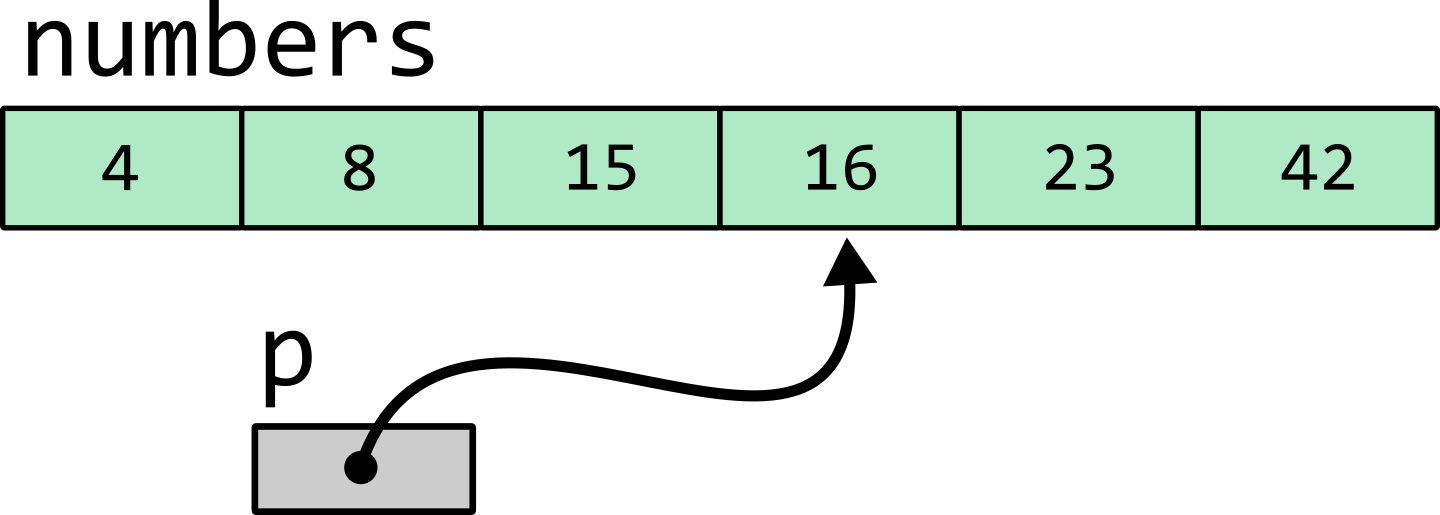
\includegraphics[scale=0.7]{../images/pointer_task_arithmetics.png}
\end{center}

Чему равны следующие выражения:
\begin{multicols}{3}
\begin{enumerate}
\item \begin{verbatim} numbers[5] \end{verbatim}
\item \begin{verbatim} *p \end{verbatim}
\item \begin{verbatim} *(p+1) \end{verbatim}
\item \begin{verbatim} *(p-2) \end{verbatim}
\item \begin{verbatim} p[0] \end{verbatim}
\item \begin{verbatim} p[1] \end{verbatim}
\item \begin{verbatim} p[-2] \end{verbatim}
\item \begin{verbatim} *numbers \end{verbatim}
\item \begin{verbatim} *(numbers+5) \end{verbatim}
\item \begin{verbatim} p - numbers \end{verbatim}
\item \begin{verbatim} (short*)p - (short*)numbers \end{verbatim}
\item \begin{verbatim} (char*)p - (char*)numbers \end{verbatim}
\end{enumerate}
\end{multicols}

Решение этой задачи -- \texttt{.txt} файл со всеми ответами.


\subsection*{Задача 10: Куб по указателю}
Напишите функцию \texttt{cube}, которая будет принимать на вход указатель, содержащий адрес некоторой переменной типа \texttt{float}. Функция должна возводиить в куб переменную, чей адрес хранит входящий указатель. Вызовите эту функцию из \texttt{main} и протестируйте её.

\subsection*{Задача 11: Умножение массива на 2}
Напишите функцию \texttt{void mult2\_array(int* p, size\_t n)}, которая принимает указатель на первый элемент некоторого массива и число \texttt{n}, равное размеру этого массива. Вам нужно, используя этот указатель, увеличить все элементы массива в 2 раза.


\subsection*{Задача 12: Квадратное уравнение}
Напишите функцию \texttt{int solve\_quadratic(double a, double b, double c, double* px1, double* px2)}, которая должна решать квадратное уравнение с коэффициентами \texttt{a}, \texttt{b} и \texttt{c}. Результат функция должна записывать по адресам \texttt{px1} и \texttt{px2}. Функция должна возвращать:
\begin{itemize}
\item \texttt{0} - если корней нет. По адресам \texttt{px1} и \texttt{px2} ничего записывать в этом случае не надо.
\item \texttt{1} - если есть один корень. Его нужно записать по адресу \texttt{px1}.
\item \texttt{2} - если есть два корня. Их нужно записать по адресам \texttt{px1} и \texttt{px2}.

Все сравнения делать с точностью $\epsilon = 10^{-10}$ .


\end{itemize}


\end{document}